\documentclass[tikz,border=12pt]{standalone}
\usepackage{amsmath}
\usepackage{amssymb}
\usepackage{tikz}
\usetikzlibrary{calc,arrows.meta,positioning}

\begin{document}
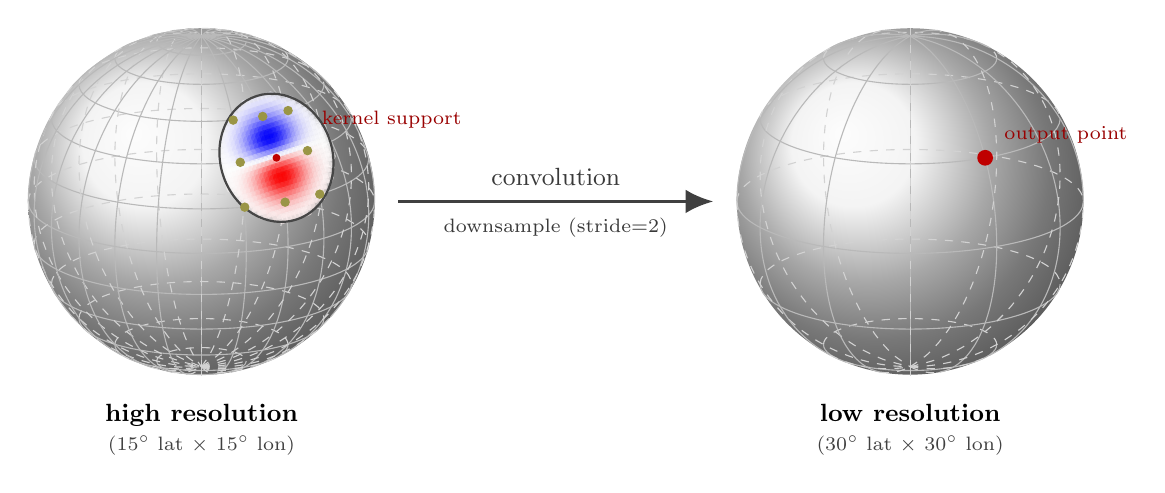
\begin{tikzpicture}[
  font=\sffamily,
  >=Latex,
  line width=0.5pt,
]

% ============================================================================
% Two equiangular-grid spheres with a downsampling arrow in between, and a
% spherical-cap "disc" drawn on the left sphere — the local DISCO conv
% kernel support that maps to a single grid point on the lower-res sphere.
%
% Convention:
%   x = right (screen), z = up (screen), y = into screen (viewer at +y).
%   Point on sphere: (R cos(lat) sin(lon), R cos(lat) cos(lon), R sin(lat))
%   Projection to 2D: drop y → (R cos(lat) sin(lon), R sin(lat)).
% ============================================================================

\def\R{2.2}                % sphere radius
\def\sep{9.0}              % horizontal distance between sphere centres
\def\sphereSq{0.30}        % magnitude of sin(β) — controls latitude-ellipse squish

% Tilt angle β. sinB < 0 means the north pole is tilted TOWARD the camera
% (so the front-visible arc of each latitude ellipse is the BOTTOM half,
% and lon=0° sits at the bottom of each lat ellipse — convention shared
% by the cap-projection code below).
\pgfmathsetmacro{\sinB}{-\sphereSq}
\pgfmathsetmacro{\cosB}{sqrt(1-\sinB*\sinB)}

% ---------- true tilted-orthographic projection of a (lat, lon) point ----------
% Camera direction d = (0, cos β, −sin β); orthographic projection drops
% the depth axis. Sets \gridXY (x-offset from sphere centre) and \gridYY (y).
\newcommand{\projGrid}[2]{%
  \pgfmathsetmacro{\gridXY}{\R*cos(#1)*sin(#2)}%
  \pgfmathsetmacro{\gridYY}{\R*cos(#1)*cos(#2)*\sinB + \R*sin(#1)*\cosB}%
}

% ---------- helper: equiangular-grid sphere ----------
% args:
%   #1 = x of sphere centre   #2 = y of sphere centre
%   #3 = lat step (degrees, must divide 90)
%   #4 = lon step (degrees, must divide 180)
\newcommand{\gridsphere}[4]{%
  % subtle ball shading
  \shade[ball color=gray!12] (#1,#2) circle ({\R});
  % --- latitude circles ---
  % Each lat=L circle projects to an ellipse centred at (cx, cy + R sin L · cos β),
  % with x-radius R cos L and y-radius R cos L · |sin β|. We draw the BOTTOM
  % half as visible (the convention for sinB<0 = north pole toward camera).
  \pgfmathtruncatemacro{\nLat}{(180-2*#3)/#3}%
  \foreach \iLat in {0,...,\nLat}{%
    \pgfmathtruncatemacro{\lat}{-(90-#3)+\iLat*#3}%
    \pgfmathsetmacro{\hh}{sin(\lat)*\R*\cosB}%
    \pgfmathsetmacro{\ww}{cos(\lat)*\R}%
    \draw[gray!55,thin] ({#1-\ww},{#2+\hh}) arc (180:360:{\ww} and {\ww*\sphereSq});
    \draw[gray!35,thin,dashed] ({#1-\ww},{#2+\hh}) arc (180:0:{\ww} and {\ww*\sphereSq});
  }
  % --- longitude meridians ---
  % Each iteration draws ONE COMPLETE great circle (the meridian at lon=φ
  % AND its anti-meridian at lon=φ+180°). Parametrising in t ∈ [-90°, 270°]
  % traces the full great circle: t ∈ [-90°, 90°] is the lon=φ half,
  % t ∈ [90°, 270°] is the anti-meridian half. Visibility flips twice along
  % this range (once where the great circle crosses the silhouette and once
  % where it crosses back); both flips occur at t = atan(cos φ · cos β / sin β)
  % and t + 180°, giving the visible interval (tA, tB) and two hidden tails.
  \pgfmathtruncatemacro{\nLon}{(180-#4)/#4}%
  \foreach \iLon in {0,...,\nLon}{%
    \pgfmathtruncatemacro{\lon}{\iLon*#4}%
    \pgfmathsetmacro{\latBndA}{atan(cos(\lon)*\cosB/\sinB)}%
    \pgfmathsetmacro{\latBndB}{\latBndA+180}%
    % visible arc
    \draw[gray!55,thin] plot[domain={\latBndA}:{\latBndB},samples=40,smooth]
      ({#1+\R*sin(\lon)*cos(\x)},
       {#2+\R*cos(\lon)*\sinB*cos(\x)+\R*\cosB*sin(\x)});
    % hidden tail near the "far" pole
    \draw[gray!35,thin,dashed] plot[domain=-90:{\latBndA},samples=15,smooth]
      ({#1+\R*sin(\lon)*cos(\x)},
       {#2+\R*cos(\lon)*\sinB*cos(\x)+\R*\cosB*sin(\x)});
    % hidden tail wrapping around to the other "far" pole
    \draw[gray!35,thin,dashed] plot[domain={\latBndB}:270,samples=15,smooth]
      ({#1+\R*sin(\lon)*cos(\x)},
       {#2+\R*cos(\lon)*\sinB*cos(\x)+\R*\cosB*sin(\x)});
  }
}

% ============================================================================
% Left sphere — HIGH resolution
% ============================================================================
\def\xL{0}
\gridsphere{\xL}{0}{15}{15}

\node[anchor=north,font=\small\bfseries] at (\xL,{-\R-0.25}) {high resolution};
\node[anchor=north,font=\scriptsize,gray!50!black]
  at (\xL,{-\R-0.65}) {(15$^\circ$ lat $\times$ 15$^\circ$ lon)};

% ---------- disc on the LEFT sphere surface (= spherical cap) ----------
% Cap centre at (lat, lon) — both must be multiples of LCM(15°, 30°) = 30°
% to land on a grid node of BOTH spheres.
\def\capLat{30}
\def\capLon{30}
\def\capAlpha{22}              % spherical-cap angular radius

% Cap centre position: visible intersection of the drawn lat/lon ellipses.
\projGrid{\capLat}{\capLon}
\pgfmathsetmacro{\capCX}{\xL + \gridXY}
\pgfmathsetmacro{\capCY}{0    + \gridYY}

% Cap boundary projection — derived for the same TILTED orthographic that
% the lat ellipses use (tilt β with sin β = \sphereSq, cos β = √(1−sq²)).
% The cap-boundary circle in 3D is the unit circle pushed through a 2×2
% linear map M = [[a,b],[c,d]] (acting on (cos θ, sin θ)) with
%   a =  cos φ
%   b = −sin L sin φ
%   c = −sin φ sin β
%   d =  cos L cos β − sin L cos φ sin β
% The semi-axes of the projected ellipse = R sin α · √(eigenvalues of MᵀM);
% the major axis direction is the eigenvector for the larger eigenvalue.
\pgfmathsetmacro{\Ma}{cos(\capLon)}
\pgfmathsetmacro{\Mb}{-sin(\capLat)*sin(\capLon)}
\pgfmathsetmacro{\Mc}{-sin(\capLon)*\sinB}
\pgfmathsetmacro{\Md}{cos(\capLat)*\cosB - sin(\capLat)*cos(\capLon)*\sinB}
\pgfmathsetmacro{\MAC}{\Ma*\Ma + \Mc*\Mc}                 % (M^T M)_11
\pgfmathsetmacro{\MBD}{\Mb*\Mb + \Md*\Md}                 % (M^T M)_22
\pgfmathsetmacro{\MABCD}{\Ma*\Mb + \Mc*\Md}               % (M^T M)_12 = (M^T M)_21
\pgfmathsetmacro{\Mtrace}{\MAC + \MBD}
\pgfmathsetmacro{\Mdet}{\Ma*\Md - \Mb*\Mc}                % det(M)
\pgfmathsetmacro{\MdiscEig}{\Mtrace*\Mtrace - 4*\Mdet*\Mdet}
\pgfmathsetmacro{\Msqrt}{sqrt(\MdiscEig)}
\pgfmathsetmacro{\LMax}{(\Mtrace + \Msqrt)/2}
\pgfmathsetmacro{\LMin}{(\Mtrace - \Msqrt)/2}
\pgfmathsetmacro{\capMajor}{\R*sin(\capAlpha)*sqrt(\LMax)}
\pgfmathsetmacro{\capMinor}{\R*sin(\capAlpha)*sqrt(\LMin)}
% Major axis direction: eigenvector (−(ab+cd), a²+c² − λ_max) of MᵀM for
% λ_max. Angle from +x of that vector.
\pgfmathsetmacro{\capAng}{atan2(\MAC-\LMax,-\MABCD)}

% --- wavelet-like function on the disc ----------------------------------------
% A dipole f(u, v) = 2u · exp(−2(u²+v²)) defined on normalised cap-tangent
% coordinates (u, v) ∈ [-1, 1] aligned with the cap's projected major/minor
% axes. Discretised onto a ~26x26 grid; each cell is a small filled disc
% whose colour saturation tracks |f|, red for f>0 and blue for f<0. The
% Gaussian envelope makes the colour fade to white at the cap edge.
\pgfmathtruncatemacro{\nGrid}{26}
\foreach \iuu in {0,...,\nGrid}{%
  \pgfmathsetmacro{\uu}{(\iuu-\nGrid/2)*2/\nGrid}%
  \foreach \ivv in {0,...,\nGrid}{%
    \pgfmathsetmacro{\vv}{(\ivv-\nGrid/2)*2/\nGrid}%
    \pgfmathsetmacro{\rrsq}{\uu*\uu+\vv*\vv}%
    \pgfmathtruncatemacro{\inDisc}{(\rrsq < 0.92) ? 1 : 0}%
    \ifnum\inDisc=1
      \pgfmathsetmacro{\fval}{3*\uu*exp(-5*\rrsq)}%
      \pgfmathsetmacro{\dotX}{\capCX+\uu*\capMajor*cos(\capAng)-\vv*\capMinor*sin(\capAng)}%
      \pgfmathsetmacro{\dotY}{\capCY+\uu*\capMajor*sin(\capAng)+\vv*\capMinor*cos(\capAng)}%
      \pgfmathsetmacro{\fmag}{min(abs(\fval)*180,100)}%
      \pgfmathtruncatemacro{\fmagInt}{\fmag}%
      \pgfmathtruncatemacro{\isPos}{(\fval > 0) ? 1 : 0}%
      \ifnum\isPos=1
        \fill[red!\fmagInt!white,opacity=0.55] (\dotX,\dotY) circle (0.07);
      \else
        \fill[blue!\fmagInt!white,opacity=0.55] (\dotX,\dotY) circle (0.07);
      \fi
    \fi
  }%
}
% Neutral outline to mark the kernel support boundary.
\begin{scope}[rotate around={\capAng:(\capCX,\capCY)}]
  \draw[gray!55!black,thick] (\capCX,\capCY) ellipse ({\capMajor} and {\capMinor});
\end{scope}

% ---------- mark every grid intersection INSIDE the disc ----------
% Spherical angular distance from a grid point (lat_G, lon_G) to the cap
% centre (capLat, capLon) is acos(sin·sin + cos·cos·cos(Δlon)). A dot is
% drawn whenever that distance is strictly between 0 and \capAlpha — so
% interior grid points get a dark-yellow marker, and the centre point
% itself is skipped (its red marker is drawn just below).
% Iteration matches the LEFT sphere's 15° lat × 15° lon grid:
%   lat = -75°, -60°, …, 75°       (i = 0..10)
%   lon =   0°,  15°, …, 165°      (i = 0..11)
\foreach \iLatG in {0,...,10}{%
  \pgfmathtruncatemacro{\latG}{-75+\iLatG*15}%
  \foreach \iLonG in {0,...,11}{%
    \pgfmathtruncatemacro{\lonG}{\iLonG*15}%
    \pgfmathsetmacro{\angDist}{acos(sin(\capLat)*sin(\latG)
                                  + cos(\capLat)*cos(\latG)*cos(\lonG-\capLon))}%
    \pgfmathtruncatemacro{\inDisc}{((\angDist < \capAlpha) && (\angDist > 0.5)) ? 1 : 0}%
    \ifnum\inDisc=1
      \projGrid{\latG}{\lonG}
      \fill[yellow!55!black] ({\xL+\gridXY},{\gridYY}) circle (0.06);
    \fi
  }%
}

% cap centre marker
\fill[red!75!black] (\capCX,\capCY) circle (0.05);

\node[anchor=south west,font=\scriptsize,red!60!black]
  at ({\capCX+0.45},{\capCY+0.25}) {kernel support};

% ============================================================================
% Right sphere — LOW resolution
% ============================================================================
\pgfmathsetmacro{\xRight}{\xL+\sep}
\gridsphere{\xRight}{0}{30}{30}

\node[anchor=north,font=\small\bfseries] at (\xRight,{-\R-0.25}) {low resolution};
\node[anchor=north,font=\scriptsize,gray!50!black]
  at (\xRight,{-\R-0.65}) {(30$^\circ$ lat $\times$ 30$^\circ$ lon)};

% highlighted output point on the right sphere — same (lat, lon) as the disc
% centre on the left sphere — placed via the same \projGrid intersection
% formula so it sits exactly on the right sphere's coarser grid node.
\projGrid{\capLat}{\capLon}
\pgfmathsetmacro{\outCX}{\xRight + \gridXY}
\pgfmathsetmacro{\outCY}{0       + \gridYY}
\fill[red!75!black] (\outCX,\outCY) circle (0.10);
\node[anchor=south west,font=\scriptsize,red!60!black]
  at ({\outCX+0.12},{\outCY+0.06}) {output point};

% ============================================================================
% Arrow between the spheres
% ============================================================================
\coordinate (ars) at ({\xL+\R+0.30},0);
\coordinate (are) at ({\xRight-\R-0.30},0);
\draw[-{Latex[length=3.5mm,width=3mm]},very thick,gray!50!black] (ars) -- (are);
\node[font=\small,anchor=south,gray!45!black]
  at ($(ars)!0.5!(are)+(0,0.08)$) {convolution};
\node[font=\scriptsize,anchor=north,gray!45!black,align=center]
  at ($(ars)!0.5!(are)+(0,-0.08)$) {downsample (stride=2)};

\end{tikzpicture}
\end{document}
